\section{Evaluation}
\label{fault_tolerance:sec:eval}

In Section~\ref{fault_tolerance:sec:methodology}, we describe our experimental methodology. In
Section~\ref{sec:proportionality}, we show that recovery from both disk and
node failure are proportional, in that the time taken to recover is
proportional to the size of the failure. In
Section~\ref{sec:scan_sharing_overhead}, we show that the overhead imposed by
scan sharing a normal job with a recovery job is low.

\subsection{Methodology}
\label{fault_tolerance:sec:methodology}

We evaluated our fault tolerance mechanisms on eight of the machines in the
cluster described in Section~\ref{sec:hardware_architecture}. Each hard drive
is configured with a single XFS partition that is configured with a single
allocation group to avoid file fragmentation across allocations groups and is
mounted with the \texttt{noatime}, \texttt{nobarrier} and \texttt{noquota}
flags set. For this evaluation, all servers were running Linux 2.6.32. Jobs
source and sink data to HDFS, configured with 128MB blocks and whole-file
replication of the primary replica of each file.

\themis is written in C++ and, in this evaluation, is compiled with
\texttt{g++} 4.7.1. The cluster coordinator, node coordinator and HDFS
rewriting proxy are written in Python.

We rely on the sort MapReduce job to evaluate our fault tolerance
mechanisms. Since sort corresponds to no-op \map and \reduce functions, it
provides a natural way of evaluating fault tolerance independently of the job
being performed. At the same time, sort's large intermediate data set size
allowed us to stress-test the system's ability to scale
proportionally. Additionally, we have found it logistically difficult to both
obtain and store freely-available data sets that are sufficiently large that
they do not fit in a single node's memory. The input data set for sort is easy
to generate synthetically, which allows us to scale the evaluation beyond a
single node.

\subsection{Proportionality of Recovery}
\label{sec:proportionality}

In this section, we explore the proportionality of our recovery process in
response to disk and node failures.

\subsubsection{Recovering From Disk Failure}
\label{sec:disk_proportionality}

\begin{figure}
  \centering
  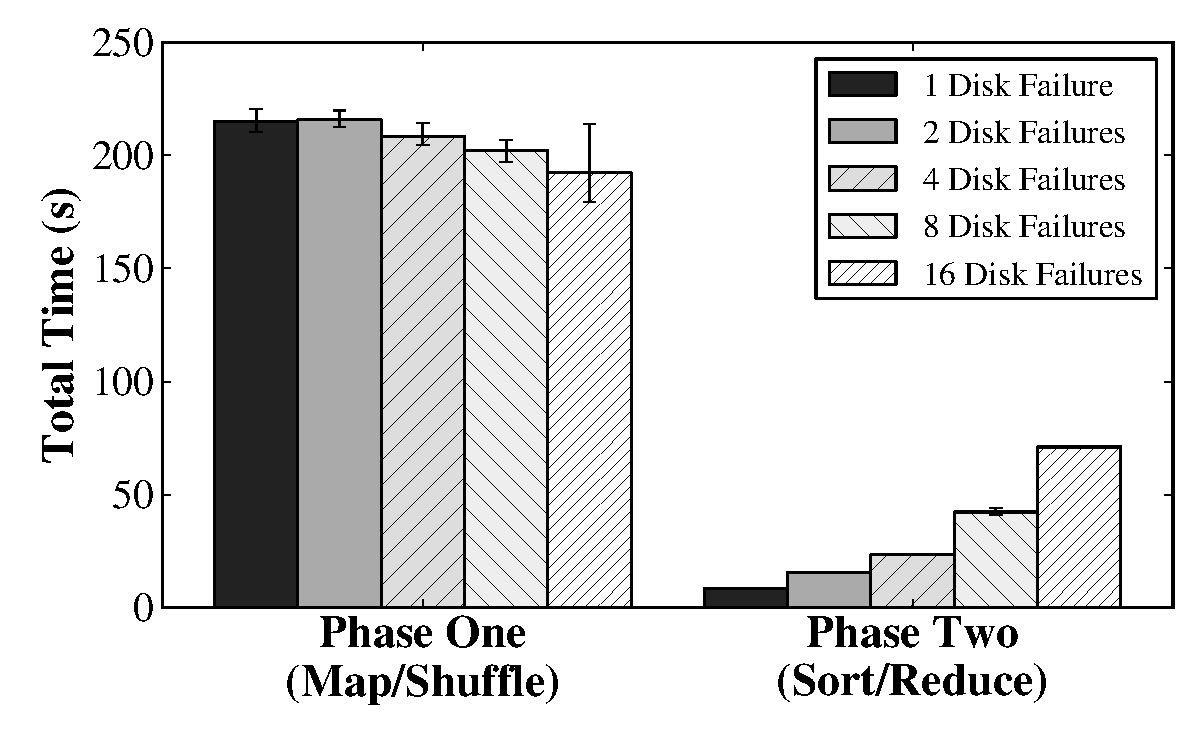
\includegraphics[width=\columnwidth]{fault_tolerance/graphs/disk_recovery_proportionality.pdf}
  \caption{\label{fig:disk_recovery_proportionality} Runtime of recovery from a
    disk failure during an 800GB sort with an increasing number of failed
    disks.}
\end{figure}

To test the proportionality of recovery from a disk failure, we ran an 800GB
sort job across our eight-node testbed and failed an increasing number of disks
during phase one. Disk failures were injected into the system by making the
part of \themis that writes to intermediate disks fail after it had written a
certain number of bytes to the disks we wanted to fail. We then ran a recovery
job to recover the data from those failed
disks. Figure~\ref{fig:disk_recovery_proportionality} shows the elapsed time of
both phases for the recovery job.

The elapsed time of the recovery job's phase two increases sub-linearly as the
number of disk failures increases.  This is because phase two is designed to
process multiple intermediate partitions in parallel and the number of
partitions created during recovery is fairly small, so processing twice as many
partitions doesn't necessarily take twice as much time. The decrease in phase
one's recovery time as the number of disks to recover increases is coincidental
and simply reflects the variability of access time provided by HDFS.

\subsubsection{Recovering From Node Failure}

\begin{figure}
  \centering
  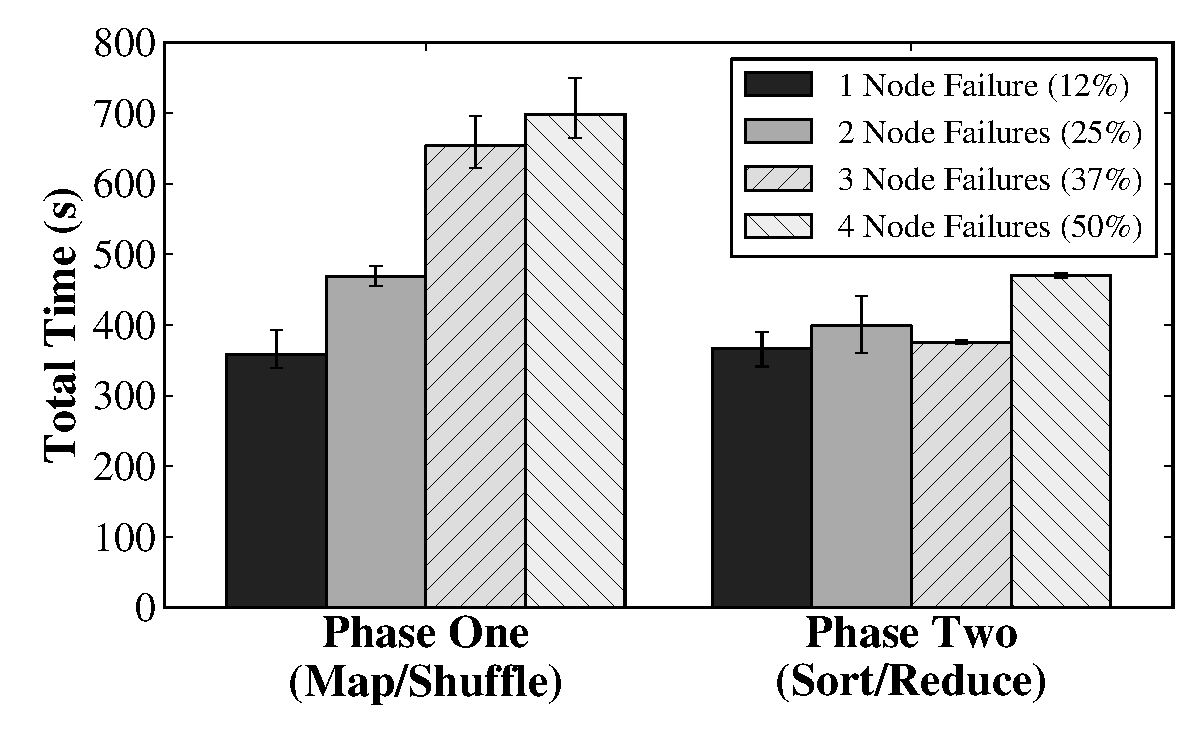
\includegraphics[width=\columnwidth]{fault_tolerance/graphs/node_recovery_proportionality.pdf}
  \caption{\label{fig:node_recovery_proportionality} Runtime of recovery from
    node failures during an 800GB sort.}
\end{figure}

To test the proportionality of recovery from node failure, we ran the same
800GB sort job as in the disk failure tests, but instead of failing individual
disks, we killed all \themis-related processes on a set of nodes approximately
120 seconds after starting the job. Each DFS disk's input consists of ten
evenly-sized files, each approximately 1.6GB
long. Figure~\ref{fig:node_recovery_proportionality} shows the elapsed time of
both phases of the recovery jobs for these failures.

Phase one's recovery time increases drastically as the number of failures
increase. The primary reason for this is that the same amount of recovery must
be done across an increasingly small number of nodes. Recovery time in phase
one is further increased by the fact that nodes are typically not accessing the
whole-file-replicated primary replica of the files they are recovering; as a
result, read performance degrades to that of unmodified HDFS.

Phase two's recovery time increases sub-linearly for the same architectural
reasons that it increases sub-linearly during disk recovery. Due to end-of-file
acknowledgments, only a small number of duplicate records are generated. As a
result, phase two's node recovery is roughly equivalent to scan-sharing phase
two of a normal 800GB sort with a disk recovery for all of the failed nodes'
disks.

\begin{figure}[t]
  \centering
  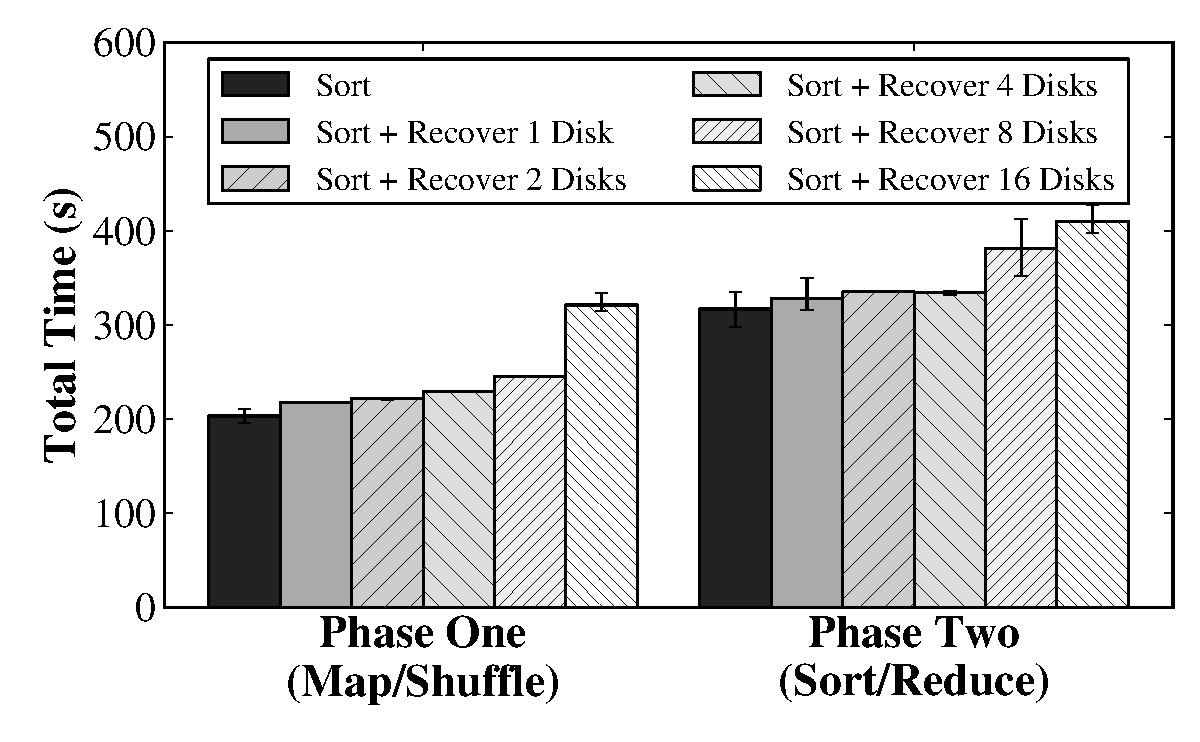
\includegraphics[width=\columnwidth]{fault_tolerance/graphs/scan_share_overhead.pdf}
  \caption{\label{fig:scan_sharing_overhead} Comparing the baseline performance
    of an 800GB sort with the performance of scan-sharing that sort with disk
    failure recovery jobs.}
\end{figure}

\subsection{Scan Sharing Overhead}
\label{sec:scan_sharing_overhead}

To evaluate the overhead imposed on a normal job by scan-sharing it with a
recovery job, we ran an 800GB sort job scan-shared with the recovery jobs
described in Section~\ref{sec:disk_proportionality}. In
Figure~\ref{fig:scan_sharing_overhead}, we see that phase one's runtime remains
fairly flat until we scan-share the sort job recovery of eight disks. At this
point, the system is writing so much intermediate data to the remaining disks
that it transitions from being bound by the speed at which it can read from
HDFS to being bound by the speed at which it can write to its intermediate
disks. At the same time, the amount of intermediate data produced by the
recovery job becomes large enough to visibly impact phase two.
